\chapter{Evaluation}

With the eventual growth of the Lightning Network a fee market for channel liquidity will emerge. How routing nodes 

\section{Lightning network as a graph}

The Lightning Network may be modeled as a directional Graph $G$ with vertices representing nodes and edges representing channels. As each channel may have different fees and liquidity in each direction it's useful to represent each channel with two edges. One edge in each direction. 

\begin{figure}[!htb]
	\hspace*{-0.7cm} 
	\centering
	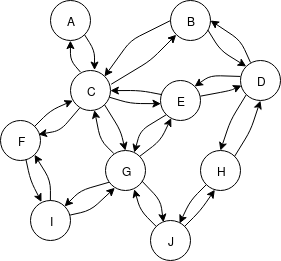
\includegraphics[width=7cm]{images/LN_overview.png}
	\caption{ \textit{A representation of LN as a graph. Each channel is symbolized by two edges.} 
	}
	\label{fig:ln:graph}
	\hspace*{2mm}
\end{figure}

Modeling the network as a graph allows the use of graph theory. Thus routing, concepts of centrality and analytical frameworks may be borrowed from the extensive literature on graphs. 

\section{Fee as a competitive equilibrium}

It may be useful to view the fee market as existing under normal free market pressures and apply the conventional long run demand and supply curve\cite{boulding:evolutionary:economy} to the fee market. 

\begin{figure}[!htb]
	\hspace*{-0.3cm} 
	\centering
	\includegraphics[width=11cm]{images/equilibrium_sized2.png}
	\caption{ The fee market as viewed according to standard price theory. Both by single pair and all pairs in aggregate. 
		}
		\label{fig:equilibrium}
		\hspace*{2mm} 	
\end{figure}

The demand curve DD' signifies users demand to utilize a shortest path in the lightning network and the supply curve the existing competing paths between s and d. Say there exists a Equilibrium point E by with the market price will move towards. Suppose the average fee price is greater than equilibrium at $F_{1}$ with demand $F_{1}D_{1}$ and supply $F_{1}S_{2}$, and more operators would open a path between s and d driving the curve fee towards E. If it instead lay under the equilibrium at $F_2$ their would be an excess supply $F_{2}S_{1}$ and low demand $F_{2}D_{2}$, making operators loose money by having liquidity locked up on a path not used. Thus leading operators to close channels between s and d, again driving the fee towards E.

The fee market may also be seen in its aggregate, where the axis represents the whole network. Here the drivers might be seen as new routing nodes joining if its a profitable venture or leaving if its a unprofitable one. Here again driving prices towards equilibrium. 

It may be unusual to view demand through the usage of its medium, their is of course a dimension here between payment systems. But there's also a the possibility of streamable payments where the say one's rent might be paid hourly or a documentary per second dependent on the fee price. With a decreased fee these payments becomes more viable driving demand.

The cost of procuring a shortest path between s and d might not be equal for two different routing nodes dependent on already existing paths and set strategies. The viability of a strategy is in essence determined in its ability to be included in shortest paths between nodes.

\section{Optimal fee price}

To determine the fee price, one could intuitively imagine that and increased fee price would yield higher fees but for less pairs as other paths may become shorter. It would be useful to have a more rigid definition of how many shortest paths pass through a vertex. Freeman did so with the introduction of a measurement named \textit{Betweenness Centrality}\cite{freeman:betweenness:centrality} and defined it as

\[ g(v) = \sum_{s \neq v \neq d}\frac{\sigma_{sd}(v)}{\sigma_{sd}} \]

Where $\sigma_{sd}$ are all shortest paths from s to d and v is vertex. As the fee is determined on an edge basis the definition is altered to regard edges instead of vertices. 

It is possible to determine the optimal fee for an edge if some assumption, of the probability of all pairs transacting and the probability of the size of the transactions, are made. If a uniform probability over all pairs and that the shortest paths are used are assumed the optimal price is given by

\[ x_{opt} \textrm{ is the optimal price } iff \]

\[ f: X \to \mathbb{Z} \textrm{ and } (\forall x \subseteq X)f(x_{opt}) \geqslant f(x) \textrm{ where }\]

\[ f(x) = x\sum_{s \neq e \neq d}\frac{\sigma_{sd}(e(x))}{\sigma_{sd}} \textrm{ and } \]

%\[ \sigma_{sd}(e(x)) =  \begin{cases}
%		n, & \text{if n shortest paths exists} \\
%          & \text{through $e$ with weight x.} \\
%		0, & \text{otherwise}
%	\end{cases} \]

\[ \sigma_{sd}(e(x)) =  \begin{cases}
 & \text{Is the sum of shortest } \\
 & \text{paths between $s$ and $d$} \\
& \text{through $e$ with weight x.} \\

\end{cases} \]


The $\sigma_{sd}$ represents the total amount of shortest paths between $s$ and $d$.
The function $f(x)$ behaves as seen in figure \ref{fig:fee_curve} for a fictitious generated graph. 

\begin{figure}[!htb]

	\centering
	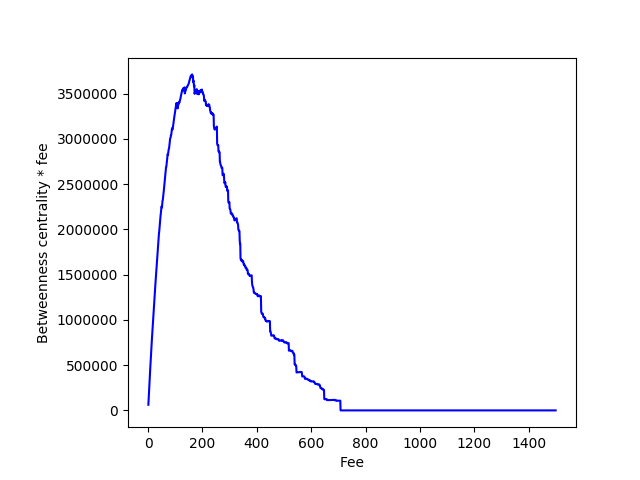
\includegraphics[width=8cm]{images/fee_curve.png}
	\caption{ Shows the betweenness centrality * fee / fee for an edge in a generated graph with 1000 vertices, 5000 edges, uniform weight distribution over 1-1500 and random attachment policy. It holds intuitively as for low fees, many shortest paths passes but procure small overall profits as the fee is small. The profits increases with the increase in fees until a point where the decrease in paths overtakes the increase in fees.
	}
	\label{fig:fee_curve}

\end{figure}

Freeman also defined a centrality measurement for whole graphs, it utilizes the betweenness centrality of every vertex and is thus brutal to calculate in practice for larger graphs. 

Efficient algorithms for edge betweenness centrality have been developed\cite{brandes:betweenness:centrality:algorithm}. Although it is possible to run such an algorithm for each potential fee price to find the optima it would be very slow.
Instead the optimal fee price an for outgoing channel $e$, still holding the assumptions as before, may be calculated by following steps.

\begin{enumerate}
	\item Calculate the shortest path from all-to-all vertices without going through $e$ with either Floyd-Warshall\cite{bakhtiar:floyd:warshall} or Johnson\cite{johnson:shortest:path:sparse:network} obtaining table A.
	\item Calculate shortest path from the source of $e$, $V$-to-all explicitly going through $e$ with Dijkstra obtaining table D where $e$ weight set to 0.
	\item Retrieve the difference for all pairs between the all-to-all distance with the all-to-$V$-to-all distance, A[s][d] - (A[s][V] + D[d]). Throw away the negative values and produce a cumulative summation over the differences in a table H.
	\item Select $x_{opt}$ such that \[ \forall x (x H(x)) \leq x_{opt} H(x_{opt}) \]
%	 producing a cumulative summation over the difference.\\
%	For all pairs s, d:\\
%		If $A[s][d] > A[s][i] + S[d]$ \\
%		then $D[A[s][d] - (A[s][i] + S[d])] += 1$.\\
	
	
		%\[ M_i := \sum_{s \neq d}^{i} A[s][d] > A[s][i] + D[d]  \]
%	\[ \sum_{s \neq d} 
%	\begin{cases}
%		A[s][d] - A[s][i] + D[d],& \text{if } A[s][d] > A[s][i] + D[d]\\
%		0,              & \text{otherwise}
%	\end{cases} \]


\end{enumerate} 

Whenever Floyd-Warshall or Johnson should be used depends on the sparseness of G as Floyd-Warshall have a time complexity of

\[ O(V^3) \]

only dependent on vertices whereas Johnson

\[ O(V^2 log(V) + VE ) \]

depends on both edges and vertices. 

\section{Topology and Preferential Attachment}

Setting fee price is only one aspect of a routing node, maybe more importantly is that of opening and closing channels.
As the protocol now stands\footnote{Is very plausible that that BIP66 may be activated allowing multi-sourced channels\cite{bip:0118:sighash:noinput}} it only allows for single source funding of channels. There is a non negligible cost to opening channels and it would be very beneficial for a node if other nodes opened channels with it instead of the other way around. This is also a prerequisite to earn profit as otherwise the node may only earn back its own funding. 

Therefor the policies determining by which preferences each node takes into account to open channels is of interest. Further these policies also affects the topology of the network, the average shortest path and robustness in case of node failures.

\subsection{Traditional random models}

Random graphs have been studied extensively, specifically the Erdős–Rényi model\cite{erdos:renyi:random:graphs}. An ER graph is created by denoting a graph $G_{n,N}$ with $n$ vertices and $N$ edges. The edges is then selected randomly from set of ${n \choose 2}$ possible edges. A common approach today is to write $G_{n,p}$ with $p$ being the probability of two vertices having an edge. It's difficult to justify LN behaving as an Erdős–Rényi graph as it allows for isolated points and there is no inherent age bias present. 

Callaway et al.~\cite{callaway:hopcraft:randomly:grown:graphs} added a phase transition to random graphs as to adjust for a supposed age bias. Consider $G_{n,\delta}$ where at first the graph is empty and for each time step a vertex v is added to the $G$ and an edge is selected over $G_v \choose 2$ with a probability $\delta$ until $G$ has $n$ vertices. $G_{n,\delta}$ would have on average $n\delta$ edges and since $n\delta < n$ it only produces sparse graphs. As before this may be difficult to apply to LN as a poorly connected graph would have high average paths and surely many payments would fail. It is however interesting to regard the degree distribution compared to that of Erdős–Rényi as it's exponential given as

\begin{equation}
	p(k) = \dfrac{(2\delta)^k}{(1 + 2\delta)^{k+1}} 
	\label{eq:callaway}
\end{equation}
compared to Erdős–Rényi which is binomial

\begin{equation}
	p(k) = {n-1 \choose k} p^k(1-p)^{n-1-k} 
	\label{eq:erdos:renyi}
\end{equation}

as follows from definition as ${n-1 \choose k}$ are all possible combinations of k edges,  $p^k$ the probability of any combination taking place and $p^k(1-p)^{n-1-k}$ to exclude combinations of larger degree $k$.

Thus adding an age bias causes the characteristics of the degree distribution to change as seen in Figure L.

\begin{figure}[!htb]
		\hspace*{-0.5cm} 
	\centering
	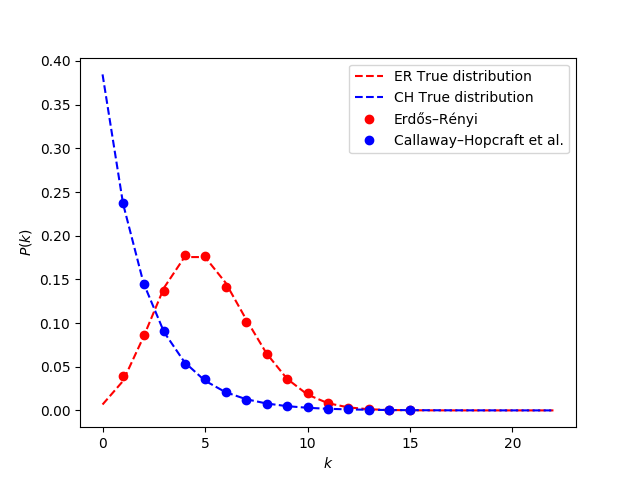
\includegraphics[width=9cm]{images/random_topology_degree_distribution.png}
	\caption{Shows the degree distribution for an Erdős–Rényi graph(\tikzcircle[blue, fill=blue]{2pt}) with n = 10,000, p = 0.0005 and its true distribution given by Equation \ref{eq:erdos:renyi}(\textcolor{blue}{|}) compared to the degree distribution for a Callaway et al. graph(\tikzcircle[red, fill=red]{2pt})  with n = 10,000, $\delta$ = 0.8 and its true distribution given by equation\ref{eq:callaway}(\textcolor{red}{|}).
	}
	\label{fig:fee_curve}
		\hspace*{2mm} 
\end{figure}

A more appropriate random model may be to consider $G_{n,m}$ where each time step $t$ a vertex is added to the graph and is connected with $m$ previous vertices and creates and edges when t < n. The probability of any previous vertex $i$ being selected is thus $p_i = \dfrac{m}{t_i}$. 
As a node may not be viewed as part of LN before edges are made, it's reasonable to assume a node creates edges as part of joining the network.

%[p(k) =  \begin{cases}
%& \prod_{i=1}^{k} 1 - \sum_{j=1}^{n-1} m \dfrac{1}{n^2},~\text{if}~m<k\\
%& 0,~~~~~~~~~~~~~~~~~~~~~~~~~\text{otherwise}

%\end{cases} \]

%\[ \prod_{i=1}^{k} 1 - \sum_{j=1}^{n-1} m \dfrac{1}{n^2} \sim 1 - m^k(\dfrac{1}{2})^k\]

\subsection{Scale free models}

In 1999 Barabási and Albert showed that many networks degree distribution follows a power law and that the distribution was independent from scale, thus scale free\cite{barabasi:albert:emergent:scaling}. Scale free networks follows a degree distribution of

\begin{equation}
	 p(k) \propto k^{-\gamma} 
	\label{eq:scale:free}
\end{equation}

and large network has been shown to follow this model. With notable networks of web hyperlinks having $\gamma_{www} = 2.1\pm 0.1$ and an actor collaboration graph having $\gamma_{actor} = 2.3\pm0.1$.
A model was suggested to generate a scale free graph by having a graph $G_{n, m}$   

preferential attachment, where a vertex prefer to connect to a vertex that already have many connections. 

\[ p_i = \dfrac{k_i}{\sum_{j}^{}k_j}  \]

\begin{figure}[!htb]
	\hspace*{-0.5cm} 
	\centering
	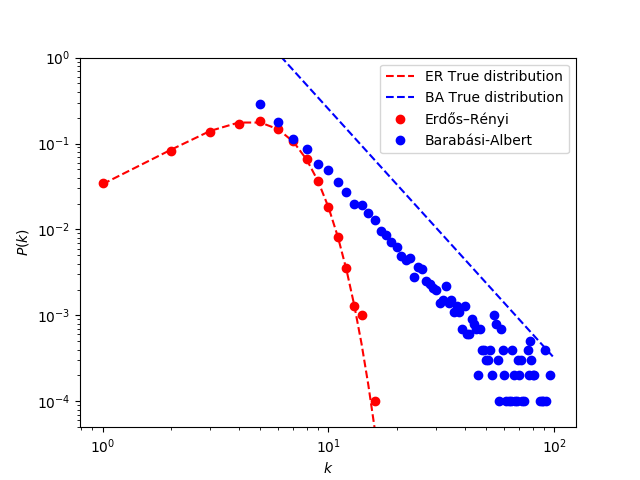
\includegraphics[width=9cm]{images/scale_free_degree_distribution.png}
	\caption{Shows the degree distribution for an Barabási–Albert graph(\tikzcircle[red, fill=red]{2pt}) with n = 10,000, m = 5 and the scale free\ref{eq:scale:free}(\textcolor{red}{|}) with $\gamma$ = 2.9 compared Erdős–Rényi graph(\tikzcircle[blue, fill=blue]{2pt}) with n = 10,000, p = 0.0005 and its true distribution given by Equation \ref{eq:erdos:renyi}(\textcolor{blue}{|}).
	}
	\label{fig:fee_curve}
	\hspace*{2mm} 
\end{figure}

modified barabasi

lightnign 

btc mainnet testnet degree distribution

The topology of both testnet and mainnet is visualized in Figure \ref{fig:topology}.

\newpage
\onecolumn

\begin{figure}[!htb]
	\hspace*{-0.7cm} 
	\centering
	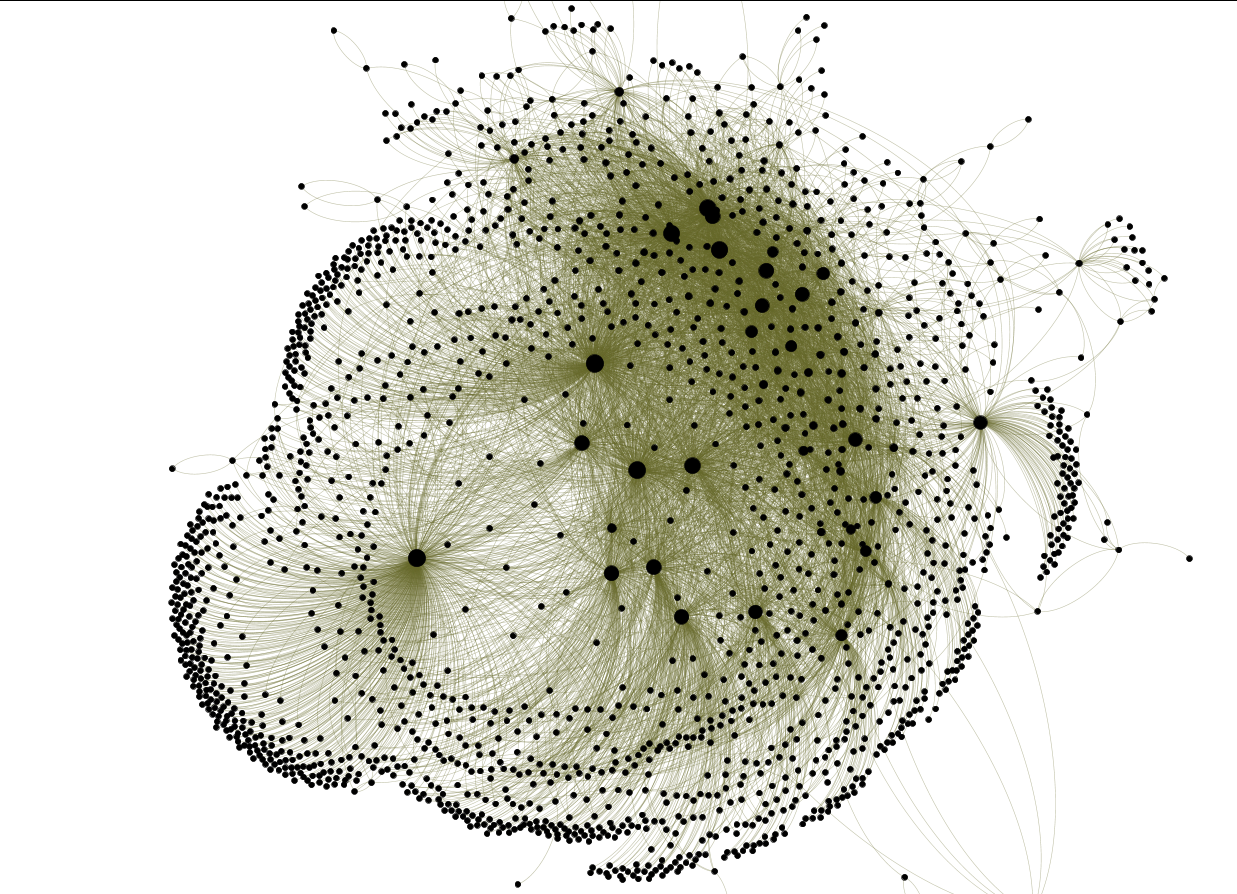
\includegraphics[width=12cm]{graphs/testnet_force.png}
	\vspace*{-0.4cm} 
	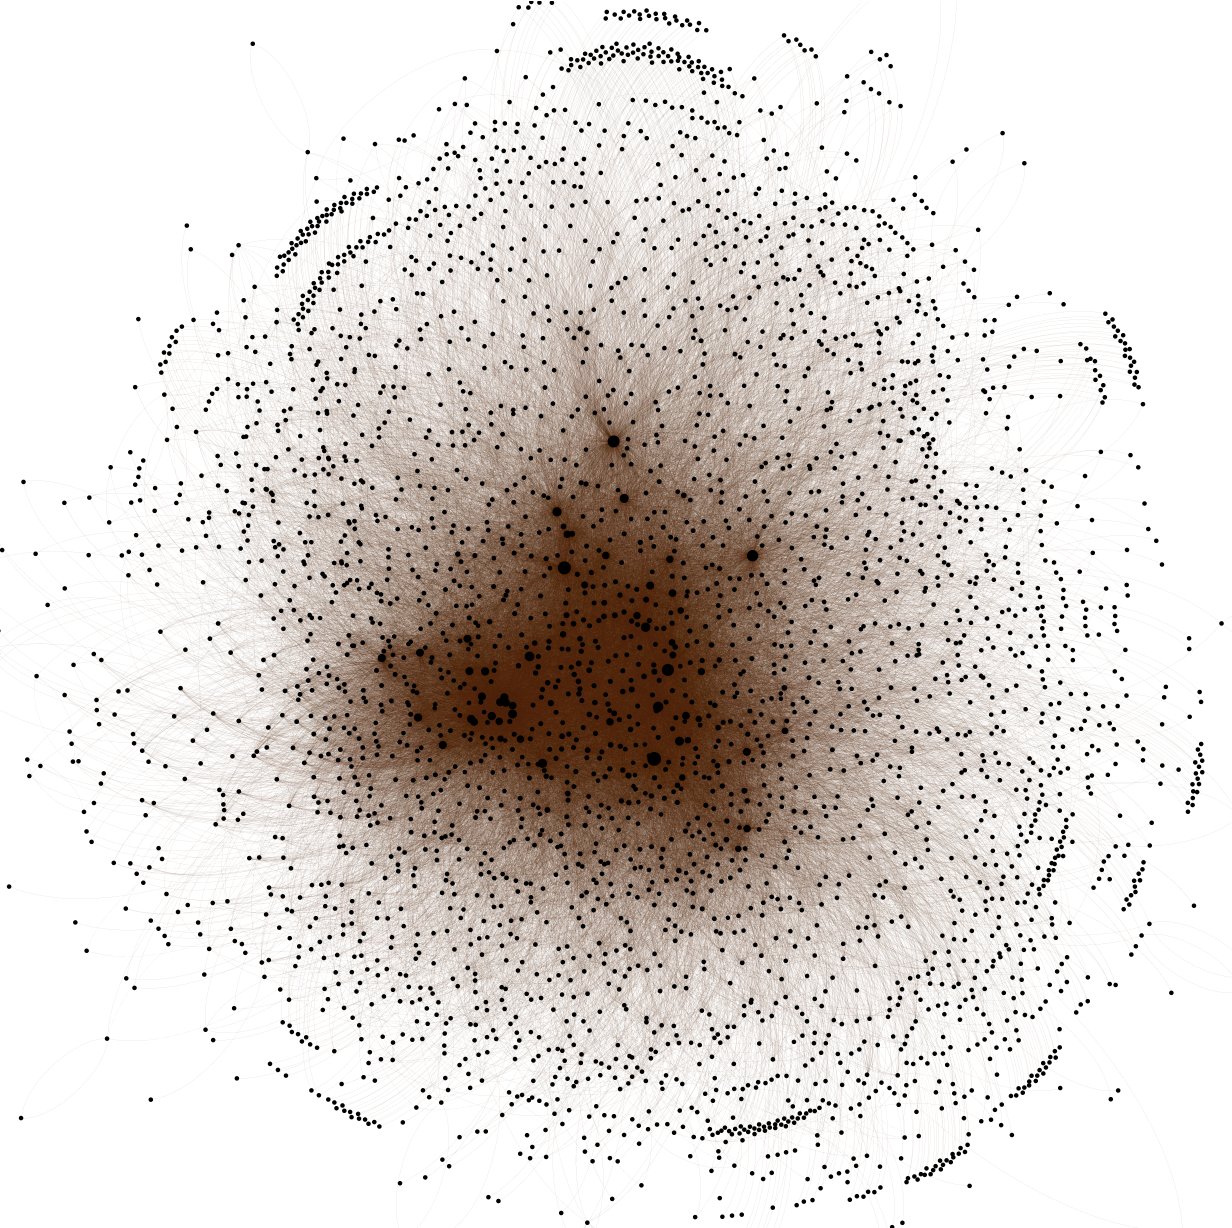
\includegraphics[width=13.6cm]{graphs/mainnet_force3.png}
	\caption{\textit{
			Shows testnet above and mainnet below as of 2019-02-25. Node size corresponds to degree, larger degrees to larger size. Positioning is a mix between Force Atlas and Fruchterman Raingold. Network data retrieved by running a c-lightning node and visualized with Gephi\cite{repository:gephi}.}}
	\label{fig:topology}
	\hspace*{2mm} 	
\end{figure}
\newpage
\twocolumn

\section{Routing as a Game}

Lightning network consists of nodes playing game

Non routing nodes, cheap as possible and possible as private as possible(?) 

does any channel opening algorithm perform better than another and essentially force the network into a scale free hub-spoke network instead of a mesh network?

\section{Simulation}

% THE ADJUSTABLE SCALE FREE  http://www.uvm.edu/pdodds/files/papers/others/2002/holme2002a.pdf

% https://webusers.imj-prg.fr/~ricardo.perez-marco/publications/articles/antrouting3.pdf

% https://bitfury.com/content/downloads/whitepaper_flare_an_approach_to_routing_in_lightning_network_7_7_2016.pdf